%\documentclass[12pt]{article}
\documentclass[aip,jcp,preprint,superscriptaddress,floatfix]{revtex4-1}
\usepackage{url,graphicx,tabularx,array,geometry,amsmath,listings}
\setlength{\parskip}{2ex} %--skip lines between paragraphs
\setlength{\parindent}{20pt} %--don't indent paragraphs

\usepackage[colorinlistoftodos,prependcaption,textsize=tiny]{todonotes} %--TODO notes

\setlength{\headheight}{-50pt}
\setlength{\textheight}{700pt}
\setlength{\textwidth}{500pt}
\setlength{\oddsidemargin}{-10pt}
\setlength{\footskip}{50pt}
\usepackage{graphicx}% Include figure files
\usepackage{bm}
\usepackage{url}
\usepackage[colorlinks = true,
            linkcolor = blue,
            urlcolor  = blue,
            citecolor = blue,
            anchorcolor = blue]{hyperref}
\graphicspath{{./Figures/}}

%-- Commands for header
\renewcommand{\title}[1]{\textbf{\large{#1}}\\}
\renewcommand{\line}{\begin{tabularx}{\textwidth}{X>{\raggedleft}X}\hline\\\end{tabularx}\\[-0.5cm]}
\newcommand{\leftright}[2]{\begin{tabularx}{\textwidth}{X>{\raggedleft}X}#1%
& #2\\\end{tabularx}\\[-1cm]}

%\linespread{2} %-- Uncomment for Double Space
\begin{document}

\title{\center{Monte Carlo Simulation of the Lennard Jones Fluid in the Canonical Ensemble}}
\rule{\textwidth}{1pt}
\leftright{The Molecular Sciences Software Institute}{Eliseo Marin-Rimoldi and John D.~Chodera} %-- left and right positions in the header

\bigskip

\section{Introduction}
\subsection{Monte Carlo Integration}

In statistical mechanics, we are interested in computing averages of
thermodynamic properties as a function of atom positions and momenta~\cite{Tuckerman.Book,Hill.Book,McQuarrie.Book}.
A thermodynamic average depending only on configurational properties can be computed using the following
expectation value integral
\begin{equation}
	\left<Q\right> = \int_V Q\left(\textbf{r}^N\right)
	\rho\left(\textbf{r}^N\right) d\textbf{r}^N
	\label{eq.statMechAverage}
\end{equation}
$\textbf{r}^N$ is a $3N$ dimensional vector containing the positions of the $N$ atoms,
where $Q(\textbf{r}^N)$ is the thermodynamic quantity of interest that depends only on the configuration $\textbf{r}^N$, 
$\rho\left(\textbf{r}^N\right)$ is the probability
density whose functional form depends on the statistical mechanical ensemble
of interest, and $V$ defines the volume of configuration space over which $\rho$ has support. 
Note that the integrals over momenta have been factored out, as
they can be evaluated
analytically. The integral (Eq.~\ref{eq.statMechAverage}) is very hard to compute
even for small atomic systems.
For instance, a monoatomic system of 10 atoms leads to a 30-dimensional
integral. Consequently, we need to resort to a numerical integration scheme if we want to
study atomic systems.

Monte Carlo methods are numerical techniques
frequently used to estimate complex multidimensional
integrals which otherwise
 could not be performed~\cite{Liu.Book,Newman.Book}.
 For instance, the integral of the function $f(\textbf{x})$,
 where $\textbf{x} \in \Re^{M}$, is approximated as
 \begin{equation}
	 I = \int_V f(\textbf{x}) \, d\textbf{x} = \int_V
	 \frac{f(\textbf{x})}{h(\textbf{x})} h(\textbf{x}) \, d\textbf{x} 
	 = \left< \frac{f(\textbf{x})}{h(\textbf{x})} \right>_{h(\textbf{x})}
	 \label{eq.averageGeneral}
 \end{equation}
 The idea of Monte Carlo integration is to estimate the expectation value
 $\left<\frac{f(\textbf{x})}{h(\textbf{x})}\right>_{{h(\textbf{x})}}$ by
 generating random samples of \textbf{x} from the probability density $h(\textbf{x})$. 

\subsection{Importance Sampling}

In Equation \ref{eq.averageGeneral}, we are free to chose the probability
distribution
$h(\textbf{x})$. The simplest case is to uniformly generate $\textbf{x}$
in the volume $V$. In this way, $h(\textbf{x})$ becomes constant as
\begin{equation}
	h(\textbf{x}) = \frac{1}{V}
	\label{eq.uniformDist}
\end{equation}
Using this sampling density $h(\textbf{x})$, the integral (Eq.~\ref{eq.averageGeneral}) becomes
\begin{equation}
	I = \int_V f(\textbf{x}) \, d\textbf{x} \approx \frac{V}{N} \sum_{i=1}^N
	f(\textbf{x}_i)
	\label{eq.averageUniform}
\end{equation}
where N is the total number of random samples and $f(\textbf{x}_i)$ is the
integrand evaluated using the $i^{th}$ sample. While using a
uniform sampling density often works sufficiently well for simple unidimensional cases, it generally fails to produce useful estimates
for complex problems.

The problem at hand involves the evaluation of $3N$-dimensional integral Eq.~\ref{eq.statMechAverage}, which is dominated by a small region of configuration space~\cite{Tuckerman.Book,Hill.Book,McQuarrie.Book}. 
Using a uniform probability distribution $h(\textbf{r}^N)$ over the configuration space hypervolume $V^{3N}$ to generate
representative samples of this subset is not efficient,
as most states generated this way would have a low weight.

A solution to this problem is to sample positions $\textbf{r}^N$ from the desired equilibrium probability density $\rho\left(\textbf{r}^N\right)$:
\begin{eqnarray}
	\textbf{r}^N &\sim& \rho(\textbf{r}^N)
\end{eqnarray}
This is a way to generate
relevant configurations more frequently than configurations that have low
probability.
Mathematically, we set $h(\textbf{r}^N)=\rho\left(\textbf{r}^N\right)$.
This idea is known as \textit{importance sampling}.

Combining Eqs.~\ref{eq.statMechAverage} and \ref{eq.averageGeneral}
and the condition $h(\textbf{r}^N)=\rho\left(\textbf{r}^N\right)$,
we find that
\begin{equation}
	%\left<Q\right> = \frac{\int Q e^{-\beta U\left(\textbf{r}^N\right)}
	%d\textbf{r}^N}{\int e^{-\beta U\left(\textbf{r}^N\right)}
	%d\textbf{r}^N}
	\left<Q\right> \approx \frac{1}{N} \sum_{i=1}^N Q\left(\textbf{r}_i^N\right) .
	\label{eq.importanceSamplingAverage}
\end{equation}
Thus, we can get thermodynamic properties by simply computing an unweighted sample average, given
that we perform importance sampling from $h(\textbf{r}^N)=\rho\left(\textbf{r}^N\right)$.

\subsection{Detailed Balance Condition}

The question now becomes how to generate such atomic positions $\textbf{r}^N$
(or \textit{states}) distributed
according to $\rho\left(\textbf{r}^N\right)$. In 1953, Metropolis, Rosenbluth, Rosenbluth, and Teller introduced a
solution based on Markov chains~\cite{Metropolis.JCP.21.1087.1953}. 
They proposed to use the detailed balance
condition in order to ensure proper configurational sampling from
the statistical mechanical distribution of interest. In order to generate
a new configuration $n$ from an old configuration $m$,
the detailed balance condition is

\begin{equation}
	\rho_m\left(\textbf{r}^N\right) \alpha \left(m \rightarrow n \right)
	P_{acc} \left(m \rightarrow n \right) =
	\rho_n\left(\textbf{r}^N\right) \alpha \left(n \rightarrow m \right)
	P_{acc} \left(n \rightarrow m \right) 
	   \label{eq.detailedBalance}
\end{equation}

Where $\rho_m\left(\textbf{r}^N\right)$ is the probability of observing
state $m$,
$\alpha \left(m \rightarrow n \right)$ is the probability of
attempting to generate a new state $n$ starting from a state $m$  and 
$P_{acc} \left(n \rightarrow m \right)$ is the probability of accepting 
such transition. Basically, the condition of detailed balance tells us that the
``flux'' of transitions
from state $m$ to state $n$ equals the flux from state $n$ to state $m$ at
equilibrium.

There are many ways to satisfy Eq.~\ref{eq.detailedBalance} by construction of different acceptance probabilities. 
While Metropolis et.~al proposed a choice that both satisfies Eq.~\ref{eq.detailedBalance} and maximizes the average acceptance probability $\left< P_{acc} \right>$~\cite{Metropolis.JCP.21.1087.1953}, Hastings generalized this to the case where proposal probabilities are not symmetric, such that $\alpha \left(m \rightarrow n \right) \ne \alpha \left(n \rightarrow m \right)$, producing the \emph{Metropolis-Hastings}~\cite{Hastings.Biometrika.57.97.1970} acceptance criteria:
\begin{equation}
	P_{acc}(m \rightarrow n) = \text{min} \left[1,\frac{\alpha \left(n
		\rightarrow m \right)}{\alpha \left(m \rightarrow n \right)}
		\frac{\rho_n\left(\textbf{r}^N\right)}{\rho_m\left(\textbf{r}^N\right)}
	\right]
	\label{eq.MetropolisHastings} .
\end{equation}
This algorithm is one of a general class of \emph{Markov chain Monte Carlo (MCMC)} algorithms that generate Markov chains to sample a desired target density, and a great deal of the MCMC literature is valuable for molecular simulations~\cite{Liu.Book}.

\section{Canonical Ensemble Monte Carlo of a Lennard Jones Fluid}

Assume we have $N$ monoatomic particles that interact using the Lennard-Jones (LJ) pairwise potential:
\begin{equation}
U(r) = 4 \epsilon \left[\left(\frac{\sigma}{r}\right)^{12} -\left(\frac{\sigma}{r}\right)^{6} \right] 
\end{equation}
where $r$ is the interparticle distance, $\sigma$ is the distance where the interaction energy is zero, and $\epsilon$ is the well depth. 
For simulating argon, for example, a common choice is $\sigma = 3.4$~\AA and $\epsilon/k_B = 120$~K.

Our goal is to generate a set of states of $N$ LJ particles distributed according to the canonical (NVT) ensemble
\begin{eqnarray}
	\rho_n \left(\textbf{r}^N ; \beta \right) &=& Z(\beta)^{-1} e^{-\beta U \left( \textbf{r}^N \right)} \label{eq:nvtDist} \\
	Z(\beta) &\equiv& \int_V e^{-\beta U \left(  \textbf{r}^N \right)} \, d\textbf{r}^N 
\end{eqnarray}
where $U \left( \textbf{r}^N \right)$ is the potential energy of the system, $\beta = (k_B T)^{-1}$ is the inverse temperature, $k_B$ is the Boltzmann constant, and $T$ is the absolute temperature. 

Note that  $U \left( \textbf{r}^N \right)$ is given by
\begin{equation}
	U \left( \textbf{r}^N \right) = \sum_{i < j} U \left( r_{ij} \right) 
	\label{eq.LennardJonesTotalPotential}
\end{equation}
where $r_{ij} \equiv || \textbf{r}^N_j - \textbf{r}^N_i ||_2$ is the interparticle separation distance.

Substituting Eq.~\ref{eq:nvtDist} into Eq.~\ref{eq.MetropolisHastings} and assuming $\alpha \left( n \rightarrow m \right) =  \alpha \left( m \rightarrow n \right)$, we obtain
\begin{equation}
	P_{acc}(m \rightarrow n) = \text{min} \left[
		1,e^{-\beta \Delta U}
	\right]
	\label{eq.detailedBalanceNVT}
\end{equation}
where $\Delta U \equiv U(\textbf{r}^N_m) - U(\textbf{r}^N_n)$ is the difference in potential energy of the system
between the new state $n$ and the old state $m$. Note that the argument
of the energy $\textbf{r}^N$ has been dropped for clarity.

\subsection{Flow of Calculations in a Metropolis Monte Carlo simulation}

The following workflow can be used to implement the Metropolis algorithm to sample the canonical ensemble of configurations of LJ particles \cite{Shell.Notes, Maginn.Notes}:

\begin{enumerate}
\setlength{\itemsep}{0em} %--don't put a huge amount of space between items in a list
\item Generate an inital system state $m$.
\item Choose an atom with uniform probability from $\{1, \ldots, N\}$ from old state $m$.
\item Propose a new state $n$ by translating a LJ particle by a uniform random displacement $\Delta r \sim U(-\Delta x, +\Delta x)$ in each dimension.
	The displacement scale $\Delta x$ should not be too large as this would
	likely result in particle overlaps, but should not be too small
	as this would result in a slow sampling of configurational space.
	More on this below.
\item The difference in energy between the new and old states is computed.
\item The new state is accepted or rejected using the Metropolis criterion.
	Practically, this can be implemented as follows. 
	If a move from $m$ to $n$ is ``downhill'', $\beta \Delta U \leq 0$,
	the move is always accepted. For ``uphill'' moves, a random
	number $\zeta$ is generated uniformly on (0,1).  
	If $\zeta < \exp[-\beta {\Delta U}]$, the move is
	accepted.  Otherwise, the move is rejected. 
	If a non-symmetric proposal is used, this acceptance scheme will have to be modified to implement Eq.~\ref{eq.MetropolisHastings}.
\end{enumerate}

\subsection{Technical considerations}

\textbf{Initial configuration.} 
While computed equilibrium expectations should be independent of the starting configuration, from a practical standpoint, we have to select an initial configuration that is not so atypical of equilibrium configurations that relaxation to equilibrium will require an enormous amount of simulation time. 
For this particular example, a good way to start is to place atoms in a 3D lattice. 
During the Metropolis Monte Carlo simulation at temperatures and box volumes (or pressures) typical of the liquid state, the lattice will ``melt'' and liquid configurations will be obtained. 
Once a liquid configuration has been generated from a simulation, you can always save a ``snapshot'' from this simulation as a starting point for a new simulation of the liquid states, and relaxation to equilibrium will generally be much more rapid as long as the conditions are similar.

\textbf{Random number generation.} 
Computers cannot generate truly random numbers.
Instead, they rely on \emph{pseudorandom number generators} (PRNGs) that aim to produce random numbers with the desired statistical properties and long recurrence times between repeats of the same random number sequence.
Using a low-quality random number generator can lead to simulation artifacts that can lead to incorrect physical behavior~\cite{Ferrenberg.PRL.69.3382.1992,Cerutti.JCTC.4.1669.2008}.
We recommend you avoid writing your own PRNGs, as this can lead to inadvertent implementation of an ill-conceived algorithm~\cite{RANDU}.
Instead, rely on high-quality, well-understood PRNGs and implementations that have are well-supported, such as the Mersenne Twister~\cite{Mersenne.Twister,Matsumoto.ACMTransModelComputSimul.8.3.1998} implementation provided by \href{https://docs.scipy.org/doc/numpy/reference/routines.random.html}{\tt numpy.random}.

\textbf{Equilibration.} 
When the initial configuration is highly atypical compared to true samples from the equilibrium density---such as the initial 3D lattice conditions compared to a true disordered liquid state---it may require very long simulation times for the bias in equilibrium averages computed over the entire trajectory to become small compared to the statistical error~\cite{Chodera.JCTC.12.1799.2016}.
It is therefore common practice to discard some initial part of the simulation to \emph{equilibration} and to average over the subsequent \emph{production} region to minimize this bias at the cost of potentially increasing statistical error by including less data in the average.
While common practice traditionally had selected an arbitrary initial portion of the simulation to equilibrium, modern best practice recommends the use of an automated approach for selecting the optimal equilibration/production split point in a manner that maximizes the number of statistically uncorrelated samples in the production part of the trajectory~\cite{Chodera.JCTC.12.1799.2016}.
To do this, you can use the \href{http://pymbar.readthedocs.io/en/latest/timeseries.html#automatically-identifying-the-equilibrated-production-region}{\tt pymbar.timeseries.detectEquilibration} function from the \href{http://pymbar.org/}{\tt pymbar} module to analyze an array containing timeseries data for your observable (such as energies, box volumes, or densities)~\cite{Chodera.JCTC.12.1799.2016}.

\textbf{System size and periodic boundary conditions.} 
A typical simulation of a Lennard-Jones fluid is carried out anywhere from 216 to 10,000 particles. 
This amount of particles is far away of being representative of a bulk liquid. 
To get around this problem, we employ a trick called periodic boundary conditions. 
The primary simulation box is surrounded
by copy images of itself. For a cubic simulation, there would be 26 
images around the central box. This trick has two implications
\begin{enumerate}
\setlength{\itemsep}{0em} %--don't put a huge amount of space between items in a list
	\item If the position of a particle (i.e.\ Cartesian coordinates) is
		outside the simulation box after a particle translation, 
		an identical particle should enter the box through the
		opposite face of the box, as shown in Figure ~\ref{fig:pbc} 
	\item When computing distances $r_{ij}$ used in the evaluation of the LJ potential (Eq.~\ref{eq.LennardJonesTotalPotential}), we use the \textit{minimum image distance}. See Figure ~\ref{fig:minimumImage}.
\end{enumerate}

\begin{figure}[t]
        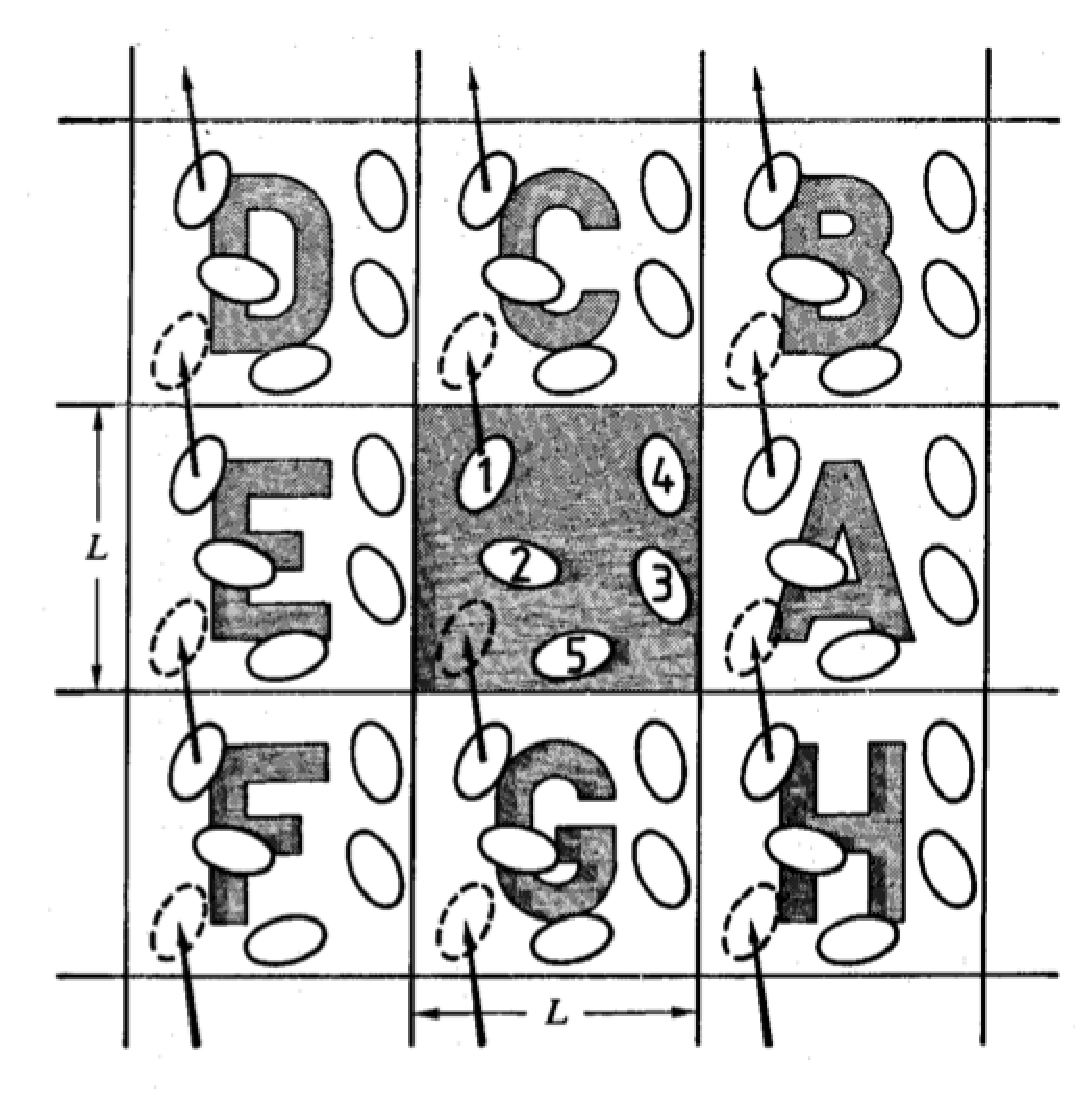
\includegraphics[scale = 0.5]{pbc.eps}
        \caption{Molecule one is displaced outside the bounds of the central box and placed back
        in through the oposite side of the box. Image from Allen and Tildesley. ~\cite{Allen.Book}}
        \centering
        \label{fig:pbc}
\end{figure}

\begin{figure}[t]
        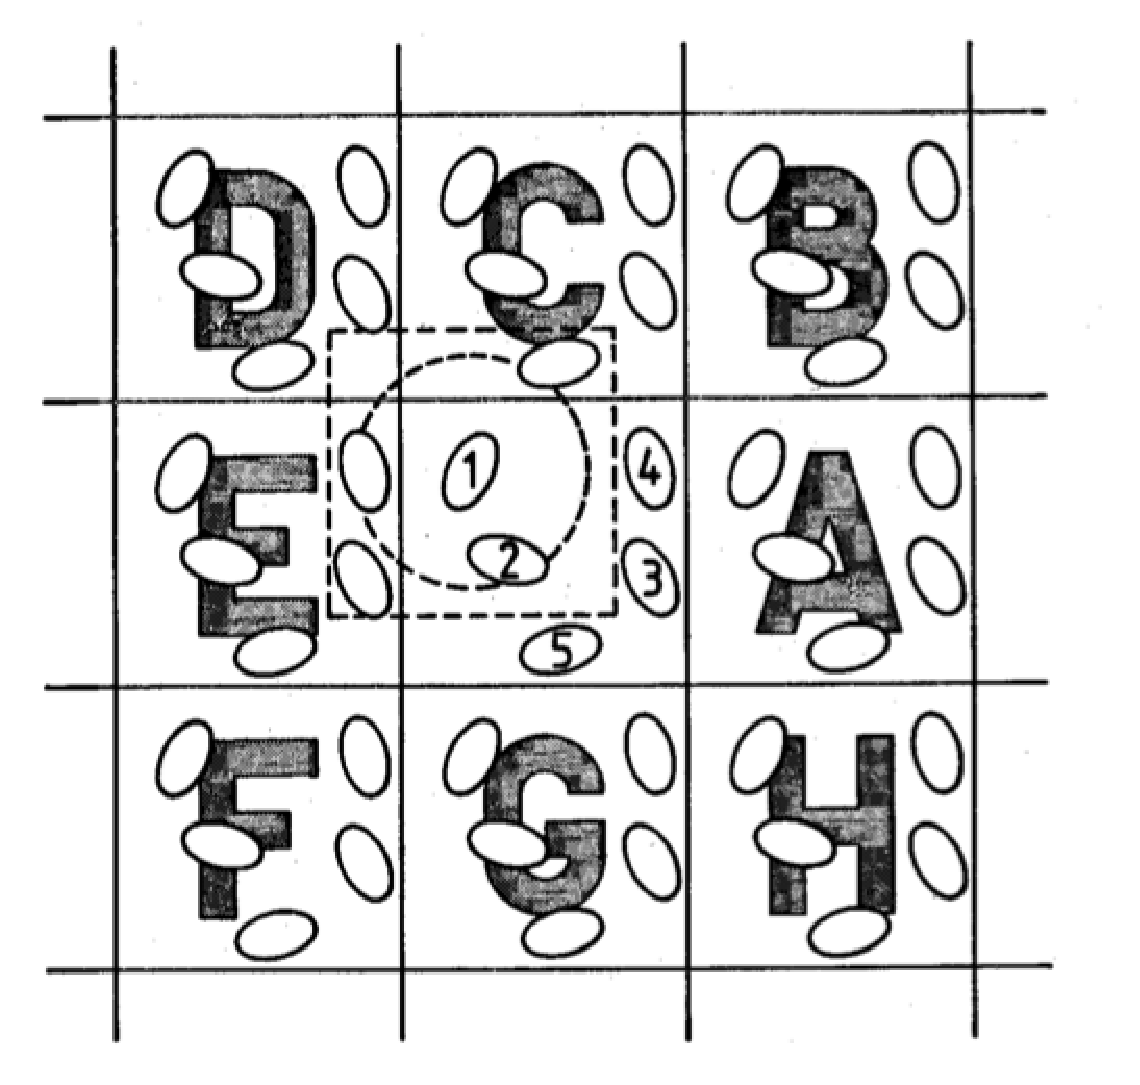
\includegraphics[scale = 0.5]{minimumImage.eps}
        \caption{Representation of the minimum image distance. Molecule 1 does not interact with
                molecule 4 located in the simulation box because the distance between particles is
                greater than the cutoff. However, molecule 1 does interact with
                the image of molecule 4 located in box E. Image from Allen and
                Tildesley ~\cite{Allen.Book}}
        \centering
        \label{fig:minimumImage}
\end{figure}

\textbf{Maximum displacement $\Delta x$.} 
As noted above, the Metropolis Monte Carlo algorithm requires translating a selected LJ particle by a random perturbation. 
This displacement should not be too large as this would result in particle overlaps and low acceptance rates; on the other hand, it should not be so small as to result in inefficient sampling of configuration space.
A common practice is to adjust the maximum particle displacement $\Delta x$ during an explicit equilibration phase in order to achieve $\sim$50\% acceptance translation rates over a recent window of $\sim N$ Monte Carlo trial moves. 

\textbf{Energy truncation and tail corrections.} 
If two particles are separatedby more than a certain distance, we typically truncate their interaction energy if $r > r_c$, where $r_c$ denotes the \emph{cutoff distance}. 
Truncating interactions removes contribution to the potential energy that might be non negligible and can lead to significant artifacts, such as significantly perturbed densities when a barostat is used to sample the NPT ensemble due to neglected long-range dispersion interactions. 
We can estimate the truncated interactions by incorporating an energy 
correction, known as the tail or long range correction.
For the Lennard-Jones fluid, we assume that we have an homogeneous liquid at $r>r_c$ to obtain the correction for neglecting this contribution for all interacting pairs of particles~\cite{Shirts.JPCB.111.13052.2007}:
\begin{equation}
	U_\mathrm{correction} = \frac{8 \pi N^2}{3 V} \epsilon \sigma^3
	\left[\frac{1}{3} \left(\frac{\sigma}{r_c} \right)^9 
	- \left(\frac{\sigma}{r_c} \right)^3 \right]
\end{equation}
For a Lennard-Jones fluid, it is common to set $r_c \sim 3 \sigma$, since the pair interaction at this separation is small, $U(3 \sigma) \approx 4 [(3)^{-12} - (3)^{-6} \approx - 0.0055 \epsilon$, or about 0.5\% of the well depth $\epsilon$.
You will want to verify that your computed properties are relatively insensitive to the choice of cutoff $r_c$ so that a too-short cutoff does not induce artifacts in computed physical properties.

\textbf{Units.}
Dealing with unit-bearing quantities---such as energies, distances, masses, and physical constants---in your code can be tricky.
Errors can easily creep in when one part of the code assumes one set of implicit units while another part of the code assumes a different set of implicit units, and error like this have led to billion-dollar accidents (such as the loss of the Mars Polar Lander due to one part of the code using metric units while the other used English units~\cite{MarsPolarLander}).
To avoid costly mistakes that complicate debugging, we recommend one of two approaches:
(1) use a unit library such as \href{http://pint.readthedocs.io/}{\tt pint} or \href{http://docs.openmm.org/7.1.0/userguide/library.html#units-and-dimensional-analysis}{\tt simtk.unit} that automatically handles unit coversions,
or (2) select a single compatible unit system (e.g.~mks or {\AA}ngstroms-amu-picoseconds) and explicitly document the units for all unit-bearing constants and quantities;
The first option is highly preferred, though care must still be paid to ensuring unit-bearing quantities possess the appropriate dimensionality and some considerations must be made for performance impact in parts of the code that must be performant since unit conversion incurs non-negligible overhead.

\textbf{Compatible constants.}
While some constants are exact, many physical constants are known only to a number of significant digits.
All values must be rounded to some number of significant figures when used in computer simulations, and these numbers have finite-precision floating-point representation that further reduces their accuracy.
Perhaps surprisingly, choices of how many significant figures that each constant should be rounded to can have an impact on the resulting simulations if care is not take to ensure that constants frequently used together are not rounded in a self-consistent manner.
For example, a major difference between potential energies computed in CHARMM and AMBER arises from an early arbitrary choice of the number of significant digits to round a set of critical Coulomb energy coefficients~\cite{Shirts.JCAMD.31.147.2017}.
Fortunately, the National Institute of Standards and Technology (NIST) provides up-to-date guidelines on consistent sets of physical parameters in the \href{http://ws680.nist.gov/publication/get_pdf.cfm?pub_id=920686}{2014 CODATA Self-Consistent Physical Constants} (updated every four years).
It is highly recommended that the CODATA parameters be adopted unless there is strong need to reproduce flawed results from a specific molecular simulation package.


\textbf{Pressure, the virial and pressure tail corrections.} To compute the system pressure,
we use the virial theorem

\begin{equation}
        P = \frac{1}{3V} \left< 3 N k_B T + \sum_{i < j} \textbf{f}_i \cdot \textbf{r}_i  \right>
\end{equation}

Where

\begin{equation}
        \sum_{i < j} \textbf{f}_i \cdot \textbf{r}_i = - \sum_{i < j} \frac{dU\left(r_{ij} \right)}{dr} r_{ij} = W
\end{equation}

The term $W$ is known as the virial and it is a pairwise sum and it can be computed
alongside the energies. Note that the negative derivative of the energy is the force.
For the LJ potential, this is

\begin{equation}
        \mathbf{f}\left(r_{ij} \right) = -\frac{dU \left(r_{ij} \right)}{dr} = - \frac{48 \epsilon}{r^2_{ij}} \left[\left(\frac{\sigma}{r_{ij}}\right)^{12} -\frac{1}{2}\left(\frac{\sigma}{r_{ij}}\right)^{6} \right] \mathbf{r}_{ij}
\end{equation}

The effect of the truncation of the interactions must be also taken into account for the pressure
computation using a correction term

\begin{equation}
        P_{tail} = \frac{16 \pi N^2}{3 V^2} \epsilon \sigma^3
        \left[\frac{2}{3} \left(\frac{\sigma}{r_c} \right)^9 
        - \left(\frac{\sigma}{r_c} \right)^3 \right]
\end{equation}




\textbf{Reduced units.}
Lennard-Jones fluids have the surprisingly pleasant behavior of possessing universal behavior when expressed in terms of \emph{reduced units} as

\begin{equation}
	U^*\left(r_{ij} \right) = 4 \left[\left(\frac{1}{r^*_{ij}}\right)^{12} -\left(\frac{1}{r^*_{ij}}\right)^{6} \right]
\end{equation}

where 

\begin{equation}
	U^* = \frac{U}{\epsilon}
\end{equation}

and 

\begin{equation}
	r^* = \frac{r}{\sigma}
\end{equation}

That is, when plotted in reduced units, all Lennard-Jones fluids exhibit the same universal behavior despite the exact choices of $\epsilon$ and $\sigma$ used in the simulation. See Table \ref{table:reducedUnits} for a list
of variables in reduced units.
Using reduced units for input and output will allow you to compare your results with others.

\begin{table}[t]
\centering
 \begin{tabular}{|c c|} 
 \hline
 Quantity & Expression \\ [0.5ex] 
 \hline\hline
 Length &  $L^*=L / \sigma$   \\ 
 Density &  $\rho^* = N \sigma^3 / V$   \\
 Energy &  $U^* = U / \epsilon$   \\
 Pressure &  $P^* = P \sigma^3 / \epsilon$   \\
 Temperature & $T^* = k_B T / \epsilon$ \\
 Volume & $V^* = V / \sigma^3$ \\
 Time & $t^* = t \sqrt{\frac{\epsilon}{m \sigma^2}}$ \\
 \hline
 \end{tabular}
 \caption{Conversion factors between real and reduced units.}
 \label{table:reducedUnits}
\end{table}

\subsection{Reference calculations}

See the following resources for NIST Lennard-Jones fluid reference data:
\begin{itemize}
\item \href{https://mmlapps.nist.gov/srs/LJ_PURE/mc.htm}{Reference thermodynamic data ($N=500$, $T^*=0.85$ and $0.90$, $r_c = 3\sigma$)}
\item \href{https://www.nist.gov/mml/csd/chemical-informatics-research-group/lennard-jones-fluid-reference-calculations}{Reference snapshot potential energies and virials}
\end{itemize}

\newpage
%
\bibliographystyle{aip.bst}
\bibliography{references.bib}

\end{document}
